% !Mode:: "TeX:UTF-8"



\chapter{项目设计}

\section{JDBC项目设计}
\subsection{开发环境}
\begin{enumerate}
    \item {开发工具} :Intellij IDEA、MySql、Navicat
    \item {STS的JDK配置} :JDK8
    \item {STS的文件编码配置} :UTF-8
\end{enumerate}


\subsection{架构模式}
基于控制台的C/S结构应用程序
\begin{verbatim}
          商家入口   管理员入口
                 \ /     
                View层
                  |
                Dao层
                  |
             Database数据库
\end{verbatim}

\begin{enumerate}
    \item 商家入口(ElmBusinessEntry):负责为商家用户提供操作入口。
    \item 管理员入口(ElmAdminEntry):负责为管理员用户提供操作入口。
    \item View层:主要负责视图层工作,为用户提供操作选项以及数据结果。
    \item Dao层:主要负责数据持久层的工作,负责与数据库进行联络的一些任务都封装在此,需要设计接口及其实现类,直接对数据库进行操作(增删改查)。
\end{enumerate}

\section{前端设计}

\subsection{项目总体设计} 

本项目就饿了么点餐系统和送货地址系统进行了实现,前端部分基于vueCli和cnpm通过vue2进行开发,并添加了font-awesome,axios,qs依赖。UI部分在项目二的基础上修改而来,使用的是html+css+javaScript进行开发。

本项目前端向后端请求接口均使用axios和post请求。页面跳转功能使用router进行路由跳转,并通过query在页面间传值。同时在vue.config.js中将端口由默认的8080修改为8081。

vueCli版本: 5.0.8

\subsection{共通组件}

\begin{enumerate}
  \item App.vue\\
  该文件为项目共通样式文件,对html和css进行了样式规范化,适用于所有组件。

  \item Footer.vue\\
  该文件将具体页面的footer部分单独独立出来,使具体页面代码更加简洁明了,避免了代码的过分重复,提供了代码的可复用性。
  
  \item Router/index.js\\
  该文件为路由文件,负责具体页面间的跳转并解决了重复路由报异常问题。
\end{enumerate}

\subsection{具体页面组件}

\begin{enumerate}
  \item Index.vue
  \begin{itemize}
    \item 页面描述
    
    饿了么项目主页,提供饿了么商家,商品搜索功能,提供外卖类别选择功能,提供了会员开通快捷入口和向用户提供推荐商家列表。本项目仅就外卖类别选择功能进行了实现。

    \item url:http://localhost:8081/
    
    \item 业务逻辑
    \begin{itemize}
      \item 外卖类别选择功能跳转到businessList界面,并将选择的外卖类别(orderTypeId)传给businessList界面。
    \end{itemize}
  \end{itemize}

  \item BusinessList.vue(这里以选择美食类别为例)
  \begin{itemize}
    \item 页面描述
    
    商家列表页面,负责向用户展示所有美食类别的可选外卖,以列表的方式呈现,提供了选择商家的功能,本项目就选择商家功能进行了实现。

    \item url:http://localhost:8081/businessList?orderTypeId=1
    
    \item 业务逻辑
    \begin{itemize}
      \item 在页面实例被创建完成后,向BusinessController/listBusinessByOrderTypeId接口发送请求,传入orderTypeId并返回该类别食品列表。然后判断用户是否登录,若登录则向CartController/listCart接口发送请求,传入userId并请求返回该用户购物车中的食品列表,将用户购物车中的对应商家对应食品数量以角标的形式在商家图片右上角展示。
      
      \item 商家选择功能跳转到businessInfo界面,并将选择的商家id(businessId)传给businessInfo界面。
    \end{itemize}
    
  \end{itemize}

  \item BusinessInfo.vue(这里以选择万家饺子为例)
  \begin{itemize}
    \item 页面描述
    
    商家信息页面,负责向用户展示选择的商家的各种信息,包括商家名称,起送费,配送费,商家提供选择的食品列表,和将食品加入购物车的功能,本项目就将食品加入购物车的功能进行了实现。

    \item url:http://localhost:8081/businessInfo?businessId=10001
    
    \item 业务逻辑
    \begin{itemize}
      \item 在页面实例被创建完成后,向BusinessController/getBusinessById接口发送请求,传入businessId并返回该商家的实体对象,将商家的信息渲染在页面上。再向FoodController/listFoodByBusinessId接口发送请求,传入businessId并返回该商家的食品列表,将列表中的食品信息渲染在页面上。然后判断用户是否登录,若登录则向后端CartController/listCart接口发送请求,传入userId和businessId并请求返回该用户购物车中该商家的食品列表,将用户购物车中的该商家的食品选择展示出来。
      \item 向购物车中添加食品功能通过向CartController/saveCart发送请求,传入businessId,userId,foodId向数据库中购物车表添加数据,并返回影响行数。如果用户没有登录,则会强制将用户路由到登录界面(login.vue)。
      \item 向购物车中删除食品功能通过向CartController/removeCart接口发送请求,传入businessId,userId,foodId向数据库中购物车表删除数据,并返回影响行数。
      \item 更新购物车中食品功能通过向CartController/updateCart接口发送请求,传入businessId,userId,foodId,quantity向数据库中购物车表修改数据,并返回影响行数。
      \item 若选购食品价格达到起送费点击去结算可跳转到确认订单(orders)界面,并将businessId传给orders界面。
    \end{itemize}

  \end{itemize}

  \item Orders.vue
  \begin{itemize}
    \item 页面描述
    
    确认订单界面,负责展示送货地址,联系人,电话号码,并向用户展示选择的食品信息,提供送货地址选择功能和去支付功能。

    \item url:http://localhost:8081/orders?businessId=10001
    
    \item 业务逻辑
    \begin{itemize}
      \item 在页面实例被创建完成后,向BusinessController/getBusinessById接口发送请求,传入businessId并返回该商家的实体对象,将商家的信息渲染在页面上。再向CartController/listCart接口发送请求,传入businessId和userId并返回用户在该商家上选择的食品信息。
      \item 选择送货地址功能跳转到userAddress界面,并将businessId传给userAddress界面。
      \item 去支付功能首先判断用户是否选择送货地址,若没有选择则禁止使用去支付功能,去支付功能向OrdersController/createOrders接口发送请求,传入userId,buisnessId,daId,orderTotal在购物车中删除数据并生成订单同时返回生成的订单编号,然后跳转到payment界面将订单编号(daId)传给payment界面。
      \end{itemize}
  \end{itemize}

  \item Payment.vue
  \begin{itemize}
    \item 页面描述
    
    在线支付页面,负责展示生成的订单的详细信息和选择支付方式并确认支付,本项目就展示订单详细信息进行了实现。

    \item url:http://localhost:8081/payment?orderId=37
    
    \item 业务逻辑
    \begin{itemize}
      \item 在页面实例被创建完成后,向OrdersController/getOrdersById接口发送请求,传入orderId并返回对应订单信息,将订单信息渲染在页面上。并实现了订单明细的隐藏与展开。
      \end{itemize}
  \end{itemize}

  \item UserAddress.vue
  \begin{itemize}
    \item 页面描述
    
    地址管理页面,展示了用户创建的地址并提供了地址的增加,修改,删除功能。

    \item url:http://localhost:8081/userAddress?businessId=10001
    
    \item 业务逻辑
    \begin{itemize}
      \item 在页面实例被创建完成后,向DeliveryAddressController/listDeliveryAddressByUserId接口发送请求,传入userId并返回数据库中用户存储的地址信息,将地址信息渲染在页面上。
      \item 地址修改功能跳转到地址修改(editUserAddress)界面,并将businessId,daId传给editUserAddress界面。
      \item 新增收货地址功能跳转到地址添加(addUserAddress)界面,并将businessId传给addUserAddress界面。
      \item 删除地址功能通过向DeliveryAddressController/removeDeliveryAddress接口发送请求,传入daId把数据库中对应的地址删除并返回影响行数。
      \item 用户点击某个地址则会返回确认订单页面(orders),并把对应的daId返回给确认订单页面,把用户选择的地址渲染出来。
      \end{itemize}
  \end{itemize}

  \item EditUserAddress.vue
  \begin{itemize}
    \item 页面描述
    
    编辑送货地址页面,在地址管理页面点击地址修改按钮即可跳转到该页面,该页面可以修改用户选择的地址的联系人姓名,性别,电话,收货地址。本项目就所有功能进行了实现。

    \item url:http://localhost:8081/editUserAddress?businessId=10001\&daId=1
    
    \item 业务逻辑
    \begin{itemize}
      \item 在页面实例被创建完成后,向DeliveryAddressController/getDeliveryAddressById接口发送请求,传入daId并返回要修改的送货地址。
      \item 地址更新功能点击更新按钮后向DeliveryAddressController/updateDeliveryAddress接口发送请求,把修改好的地址信息打包成deliveryAddress对象传入,把原地址信息修改为当前地址信息,并返回影响行数。
      \end{itemize}
  \end{itemize}

  \item AddUserAddress.vue
  \begin{itemize}
    \item 页面描述
    
    新增收货地址页面,用户可添加联系人,性别,电话,收货地址信息并保存,本项目就该功能进行了实现。

    \item url:http://localhost:8081/addUserAddress?businessId=10001
    
    \item 业务逻辑
    \begin{itemize}
      \item 保存功能通过向DeliveryAddressController/saveDeliveryAddress接口发送请求,将用户添加的收货地址信息封装到一个deliveryAddress对象中传入,实现把送货地址信息添加到数据库中,并返回影响行数,随后跳转回到地址管理页面。
      \end{itemize}
  \end{itemize}

  \item Login.vue
  \begin{itemize}
    \item 页面描述
    
    用户登录界面,提供用户输入手机号码和密码进行登录功能,和注册功能,本项目就上述所有功能进行了实现。

    \item url:http://localhost:8081/login
    
    \item 业务逻辑
    \begin{itemize}
      \item 登录功能通过向UserController/getUserByIdByPass接口发送请求,传入userId和password验证用户输入的用户名和密码是否存在与数据库中,并返回影响行数。如果车工登录,将用户的登录数据存储在sessionstorage中供其他页面调用。
      \item 去注册功能通过路由跳转到regiter.vue页面。
      \end{itemize}
  \end{itemize}

  \item Regiter.vue
  \begin{itemize}
    \item 页面描述
    
    用户注册界面,为用户提供通过输入手机号码,密码,确认密码,用户名称,性别信息进行注册的功能,本项目就该功能进行了实现。

    \item url:http://localhost:8081/register
    
    \item 业务逻辑
    \begin{itemize}
      \item 注册功能通过向UserController/saveUser接口发送请求,将用户输入手机号码,密码,用户名称数据存储在User对象中传入,向数据库中添加新用户的数据完成注册,并返回影响行数。
      \end{itemize}
  \end{itemize}

  \item OrderList.vue
  \begin{itemize}
    \item 页面描述
    
    订单列表信息,负责向用户展示未支付和已支付的订单信息。包括每一笔订单的商家名称,订单金额,订单明细等信息。

    \item url:http://localhost:8081/orderList
    
    \item 业务逻辑
    \begin{itemize}
      \item 在页面实例被创建完成后,向OrdersController/listOrdersByUserId接口发送请求,传入userId并返回数据库中用户创建的订单信息列表,遍历列表里每一笔订单的信息然后渲染在页面上。
      \end{itemize}
  \end{itemize}


\end{enumerate}

\section{Servlet后端设计}

\subsection{开发环境}

\begin{enumerate}
\item 开发工具:SpringToolSuite(STS)、MySql、MySQL Workbench
\item 检查STS的jdk配置:jdk8
\item 检查STS的tomcat配置:tomcat8.5
\item 检查STS的文件编码配置:utf-8
\end{enumerate}


\subsection{架构模式}

基于Servlet的简易MVC架构

\begin{verbatim}
                   用户层
                     |
              DispatcherServlet
                     | 
                Controller层
                     |
                  Service层
                     |
                    Dao层
                     |
                Database数据库
\end{verbatim}


\begin{enumerate}
\item DispatcherServle:前端控制器,所有匹配请求的入口,把拦截下来的请求,依据相应的规则分发到目标Controller来处理,是配置spring MVC的第一步。
\item Controller层:负责具体的业务模块流程的控制,在此层要调用service层的接口来控制业务流程,负责url映射,针对具体的业务流程,会有不同的控制器。
\item Service层:主要负责业务模块的应用逻辑应用设计,设计接口和其实现类,在Spring的配置文件中配置其实现的关联,这样我们就可以在应用中调用service接口来进行业务处理。service层的业务层具体要调用已经定义的dao层接口
\item Dao层:主要负责数据持久层的工作,负责与数据库进行联络的一些任务都封装在此,需要设计接口及其实现类,直接对数据库进行操作(增删改查)。
\end{enumerate}

\begin{verbatim}
关系:Service层是建立在DAO层之上的,建立了DAO层后才可以建立Service层,而Service层又是Controller层之下的,因而 Service层应该既调用DAO层的接口,又要提供接口给Controller层的类来进行调用,DispatcherServlet负责把请求映射到对应的controller。
\end{verbatim}



\subsection{功能及接口实现}

\begin{figure}[htbp]
\centering
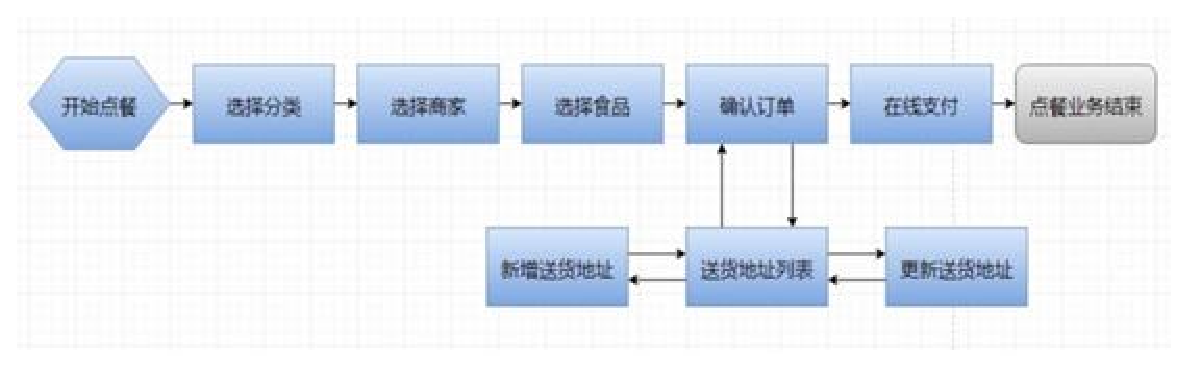
\includegraphics[width=0.8\textwidth]{progress}
\caption{点餐业务流程图}\label{fig:xml}
\vspace{\baselineskip}
\end{figure}
\begin{verbatim}
1.登录
实现方式:将输入匹配已经存在数据库user表中的userId和password,若匹配成功则登录用户。
实现接口:UserController/getUserByIdByPass

2.注册
实现方式:将注册新用户输入的信息存入数据库的user表中,向表中加一条新记录。
实现接口:UserController/saveUser

3.选择分类
实现方式:不同的分类代表着不同的orderTypeId,根据business表中属性orderTypeId查询所属business信息,返回business数组。
实现接口:BusinessController/listBusinessByOrderTypeId

4.选择商家
实现方式:将business对象封装起来,根据business表中的businessId查询business对象信息,最终返回business对象。
实现接口:BusinessController/getBusinessById

5.选择食品
功能1:呈现食品列表
实现方式:将food对象封装,在food表中businessId查询所属食品信息,最终返回food对象的数组。
实现接口:FoodController/listFoodByBusinessId

功能2:添加食品
实现方式:将食品信息、商家信息和用户信息向cart表中添加一条记录
实现接口:CartController/saveCart

功能3:在购物车中更改食品数量
实现方式:点击“+”号或“-”号,将cart表中的quantity的属性值加1或减1(值不为0)。
实现接口:CartController/updateCart

功能4: 移出购物车
实现方式:cart表中的quantity的属性值为0时,在cart表中根据userId、businessId、foodId删除该记录。
实现接口:CartController/removeCart

6.选择地址
功能1:新增地址
实现方式:将输入信息存入deliveryaddress表中,向表中添加一条记录。
实现接口:DeliveryAddressController/saveDeliveryAddress

功能2:更改地址信息
实现方式:根据daId更新送货地址的各属性值。
实现接口:DeliveryAddressController/updateDeliveryAddress

功能3:删除地址
实现方式:在deliveryaddress表中根据daId删除该daId对应的记录。
实现接口:DeliveryAddressController/removeDeliveryAddress

功能4:显示用户可选地址列表
实现方式:将deliveryAddress对象封装,在deliveryaddress表根据userId查询所属送货地址,返回deliveryAddress数组,再根据daId查询送货地址,返回deliveryAddress对象。
实现接口:DeliveryAddressController/listDeliveryAddressByUserId
DeliveryAddressController/getDeliveryAddressById

7.确认订单(在线支付)
实现方式:根据userId、businessId、orderTotal、daId向orders表中添加一条记录,并获取自动生成的orderId。然后根据userId、businessId从cart表中查询所有数据,批量添加到orderdetailet表中,然后根据用户编号、商家编号删除cart表中的数据。
实现接口:OrdersController/createOrders   
         CartController/removeCart

8.查询历史订单:
实现方式:将orders对象封装,在orders表中根据userId号查询此用户的所有订单信息,返回orders数组。根据orderId查询订单信息,包括所属商家信息,和此订单的所有订单明细信息。
实现接口:OrdersController/listOrdersByUserId  
         OrdersController/getOrdersById
\end{verbatim}


\section{SpringBoot后端设计}

\subsection{开发环境}

\begin{enumerate}
    \item 开发工具:SpringToolSuite、MySql、Navicat
    \item STS的jdk配置:jdk8
    \item Maven构建工具的配置: Maven3
    \item STS的文件编码配置:utf-8
\end{enumerate}

\subsection{架构模式}
基于Springboot+VUE-Cli的前后端分离工程

\begin{verbatim}
                用户层
                  | 
             Controller层
                  |
               Service层
                  |
                 Mapper层
                  |
             Database数据库
\end{verbatim}

\begin{enumerate}
\item Controller层:负责具体的业务模块流程的控制,在此层要调用service层的接口来控制业务流程,负责url映射,针对具体的业务流程,会有不同的控制器。
\item Service层:主要负责业务模块的应用逻辑应用设计,设计接口和其实现类,在Spring的配置文件中配置其实现的关联,这样我们就可以在应用中调用service接口来进行业务处理。service层的业务层具体要调用已经定义的dao层接口
\item Mapper层:即Dao层,主要负责数据持久层的工作,负责与数据库进行联络的一些任务都封装在此,需要设计接口及其实现类,直接对数据库进行操作(增删改查)。
\end{enumerate}

\subsection{功能及接口实现}
\begin{verbatim}
同Servlet 
    \end{verbatim}

